\documentclass{article}

\usepackage{amsmath, amssymb, geometry, multicol, tikz}
\usetikzlibrary{arrows, decorations.markings}

\tikzset
    { pointy arrow/.style = 
        { decoration = 
            { markings
            , mark=at position 1 with {\arrow[scale=1, >=latex] {>}}
            }
        , postaction = {decorate} 
        }
    }

\newcommand{\de}{\textrm{d}}

\title{Edexcel Advanced Level GCE Mathematics FP2}
\author{William Bevington \and Callum O'Brien \and Alex Pace}
\date{}

\begin{document}

\maketitle
\tableofcontents
\newpage

\section{Complex Numbers}

\subsection{De Moivre's Theorem}

De Moivre's theorem states \[z = r \left( \cos \theta + i \sin \theta \right)
\Leftrightarrow z^n = r^n \left( \cos \left( n \theta \right) + i \sin \left( n
\theta \right) \right)\] Using the exponential form, this is equivalent to \[z =
    r e^{i \theta} \Leftrightarrow z^n = \left( r e^{i \theta} \right)^n = r^n
e^{i n \theta}\]

\subsubsection{Proof of DMT}

Let $P_n$ be a predicate:\[P_n \Leftrightarrow \left( r \left( \cos \theta + i
\sin \theta \right) \right)^n = r^n \left( \cos \left( n \theta \right) + i \sin
\left( n \theta \right) \right)\] Let $n \rightarrow 1$. Evidently, \[P_1
    \Leftrightarrow r \left( \cos \theta + i \sin \theta \right) = r \left( \cos
\theta + i \sin \theta) \right)\] thus \[P_1 \text{ is True}\] Assume $P_k$:
\[\left( r \left( \cos \theta + i \sin \theta \right) \right)^k = r^k \left(
\cos \left( k \theta \right) + i \sin \left( k \theta \right) \right)\] Now,
consider $P_{k + 1}$: \[\left( r \left( \cos \theta + i \sin \theta \right)
    \right)^{k + 1} = r \left( \cos \theta \right) \times r^k \left( \cos \left(
k \theta \right) + i \sin \left( k \theta \right) \right)\] \[= r^{k +
    1} \left( \cos \left( \theta \left( k + 1 \right) \right) + i \sin
    \left( \theta \left( k + 1 \right) \right) \right) \Leftrightarrow
P_{k + 1}\] therefore \[P_k \Rightarrow P_{k + 1}\] Thus, by induction,
\[P_n \quad \forall n \in \mathbb{N} n \geq 0\]

\subsubsection{Uses}

DMT is great, because it can be used to simplify expressions like this:

\[\frac{\left(\cos\left(\frac{9\pi}{17}\right)+i\sin\left(\frac{9\pi}{17}\right)\right)^5}{\left(\cos\left(\frac{2\pi}{17}\right)-i\sin\left(\frac{2\pi}{17}\right)\right)^3}\]

\noindent First we must put the denominator into the correct polar form (with a
\(+\) inbetween cos and sin), and then we can apply de Moivre's Theorem.

\[\frac{\left(\cos\left(\frac{9\pi}{17}\right)+i\sin\left(\frac{9\pi}{17}\right)\right)^5}{\left(\cos\left(\frac{-2\pi}{17}\right)+i\sin\left(\frac{-2\pi}{17}\right)\right)^3}\]

\noindent And now appying de Moivre's Theorem:

\[\frac{\cos\left(\frac{45\pi}{17}\right)+i\sin\left(\frac{45\pi}{17}\right)}{\cos\left(\frac{-6\pi}{17}\right)+i\sin\left(\frac{-6\pi}{17}\right)}\]

\noindent From this point we can easily simplify the complex number down.

\[\cos\left(\frac{51\pi}{17}\right)+i\sin\left(\frac{51\pi}{17}\right)\]

\[\cos\left(3\pi\right)+i\sin\left(3\pi\right)\]

\[\cos\left(\pi\right)+i\sin\left(\pi\right)=-1\]

\subsubsection{De Moivre's Theorem and Trigonometric Identities}

De Moivre's Theorem can also be applied to problems consisting of trigonometric
functions by using identites and binomial expansion. First though, it is worth
noting the following, where \(Z\) is a complex number
\(r\left(\cos\left(\theta\right)+i\sin\left(\theta\right)\right)\)

\[\begin{array}{cc} 
            \vspace{15pt} Z+\frac{1}{Z} \:=\: 2\cos\left(\theta\right) \hspace{10pt} & Z^n+\frac{1}{Z^n} \:=\: 2\cos\left(n\theta\right) \\
            Z-\frac{1}{Z} \:=\: 2i\sin\left(\theta\right) \hspace{10pt} &  Z^n-\frac{1}{Z^n} \:=\: 2i\sin\left(\theta\right)
\end{array}\]

\noindent Trigonometric functions can be replaced with these arrangements of
complex numbers and then manipulated far more easily. The following is an
example of such a situation. \\


\noindent Express \(\sin^3\left(\theta\right)\) in the form
\(d\cos\left(4\theta\right)+e\cos\left(2\theta\right)+f\)

\[Z-\frac{1}{Z} \:=\: 2i\sin\left(\theta\right) \;\therefore\;
\left(Z^4-\frac{1}{Z^4}\right)^4 \:=\: 16\sin\left(4\theta\right)\]
\[\left(Z^4-\frac{1}{Z^4}\right)^4 \:=\:
Z^4+4Z^3\left(\frac{-1}{Z}\right)+6Z^2\left(\frac{-1}{Z}\right)^2+4Z\left(\frac{-1}{Z}\right)^3+\left(\frac{-1}{Z}\right)^4\]
\[\rightarrow\: Z^4+4Z^2+6-4Z^{-2}+Z^{-4}\] \[\rightarrow\:
\left(Z^4+\frac{1}{Z^4}\right)-4\left(Z^2+\frac{1}{Z^2}\right)+6\]
\[\therefore\: 16\sin^4\left(\theta\right) \:=\:
2\cos\left(4\theta\right)-8\cos\left(2\theta\right)+6\] \[\therefore\:
\sin^4\left(\theta\right) \:=\:
\frac{1}{8}\cos\left(4\theta\right)-\frac{1}{2}\cos\left(2\theta\right)+\frac{3}{8}\]

\subsubsection{Finding the $n$\textsuperscript{th} Root of a Polynomial Using De
Moivre's Theorem}

Solve \(Z^3=1\). Represent Solutions on an argand diagram.

\[|Z^3|=1 \;\; arg(Z^3)=\pi\]
\[Z^3=1\left(\cos\left(\pi\right)+i\sin\left(\pi\right)\right)\]
\[Z^3=\left(\cos\left(\pi+2k\pi\right)+i\sin\left(\pi+2k\pi\right)\right)\]
\[Z=\left(\cos\left(\pi+2k\pi\right)+i\sin\left(\pi+2k\pi\right)\right)^{\frac{1}{3}}\]
\[Z=\cos\left(\frac{\pi+2k\pi}{3}\right)+i\sin\left(\frac{\pi+2k\pi}{3}\right)\]

\noindent We only need consider all values of k for which \(\pi<\theta<\pi\)

\[k=0 \;\rightarrow\; Z=\cos\left(\frac{\pi}{3}\right)+i\sin\left(\frac{\pi}{3}\right)\]
\[\therefore \; Z \:=\: \frac{1}{2}+\frac{\sqrt{3}}{2}i\]
\[k=1 \;\rightarrow\; Z=\cos\left(\pi\right)+i\sin\left(\pi\right)\]
\[\therefore \; Z \:=\: -1\]
\[k=-1 \;\rightarrow\; Z=\cos\left(\frac{-\pi}{3}\right)+i\sin\left(\frac{-\pi}{3}\right)\]
\[\therefore \; Z \:=\: \frac{1}{2}-\frac{\sqrt{3}}{2}i\]

\begin{figure}[h]

    \centering

    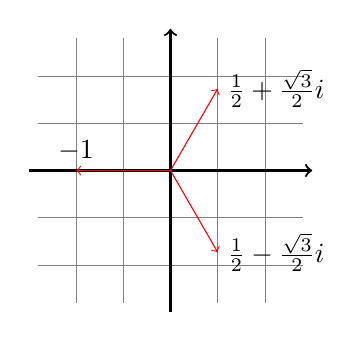
\begin{tikzpicture}[xscale=1.2,yscale=1.2]

        \draw[help lines, step=0.5] (-1.4, -1.4) grid (1.4, 1.4);
        \draw[thick, ->] (-1.5, 0) -- (1.5, 0);
        \draw[thick, ->] (0, -1.5) --(0, 1.5);

        \draw[red, ->] (0,0) -- (-1,0);
        \draw[red, ->] (0,0) -- (0.5,0.866);
        \draw[red, ->] (0,0) -- (0.5,-0.866);
        
        \draw[anchor=south] (-1,0) node {\(-1\)};
        \draw[rotate=60, anchor=west] (1, 0) node {\(\frac{1}{2} +
        \frac{\sqrt{3}}{2}i\)}; 
        \draw[rotate=-60, anchor=west] (1, 0) node {\(\frac{1}{2} -
        \frac{\sqrt{3}}{2}i\)};

    \end{tikzpicture}

    \caption{Third roots of $-1$ shown on an argand diagram} 

\end{figure}

\section{Polynomial Expansions}

Maclaurin's expansion is a way to fit a polynomial to an arbitrary function. It
states \[f(x) \approx f(0) + xf'(0) + \frac{x^2f''(0)}{2} +
    \frac{x^3f'''(0)}{6} + \cdots + \frac{x^nf^n(0)}{n!} = \sum_{r=0}^{n}
\frac{x^rf^r(0)}{r!}\] Mapping this out to infinite terms gives an exact
equivalence, called a Maclaurin series; \[f(x) = \sum_{r_0}^{\infty}
\frac{x^rf^r(0)}{r!}\]

\section{Polar Coordinates}

\begin{multicols}{2}

    \begin{center}

        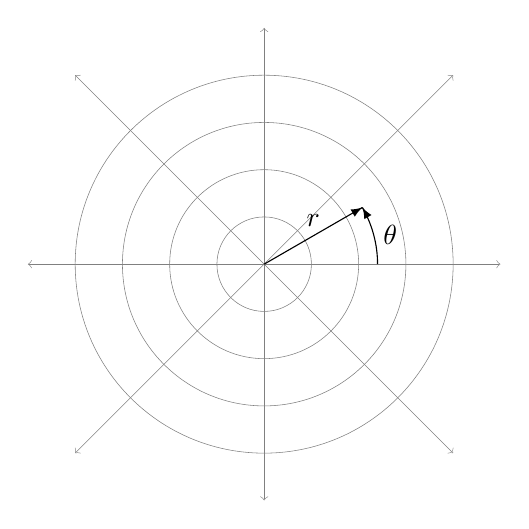
\begin{tikzpicture}[scale=1.2]

            \foreach \x in {0, 0.5, ..., 2} \draw[help lines] (0, 0) circle (\x);
            \draw[help lines, <->] (-2, -2) -- (2, 2);
            \draw[help lines, <->] (2, -2) -- (-2, 2);
            \draw[help lines, <->] (0, -2.5) -- (0, 2.5);
            \draw[help lines, <->] (-2.5, 0) -- (2.5, 0);

            \draw[pointy arrow] (1.2, 0) arc (0:30:1.2);
            \draw[rotate=15, anchor=west] (1.2, 0) node {$\theta$};

            \draw[rotate=30, pointy arrow] (0, 0) -- (1.2, 0);
            \draw[rotate=30, anchor=south] (0.6, 0) node {$r$};

        \end{tikzpicture}

    \end{center}

    \noindent Points in a space described by polar coordinates are defined in
    terms of the magnitude and direction of their displacement from the origin.
    In a two dimensional space, \(\left( r, \theta \right)\) is an arbitrary
    point, where either \(\theta \in (-pi, \pi \,]\) or \(\theta \in [\, 0, 2
    \pi)\). This is equivalent to \((x, y)\), the cartesian form, where \[x = r
    \cos \theta, \quad y = r \sin \theta\] \[r = \left( x^2 + y^2
        \right)^{\frac{1}{2}}, \quad \theta = \arctan \left( \frac{y}{x}
    \right)\] Cartesian equations can hence be converted into equivalent polar
    equations and vice versa. 

\end{multicols}

\section{Differential Equations}

\subsection{First Order Linear Inhomogeneous Ordinary Differential Equations}

First order linear inhomogeneous ordinary differential equations can be
expressed in the form \[\frac{\de y}{\de x} + P(x)y = Q(x)\]

\end{document}
